\chapter{D\'EROULEMENT DE L'AUDIT}

\section*{7.1 Chronologie}
\addcontentsline{toc}{section}{7.1 Chronologie}
\begin{table}[H]
\centering
\caption{Chronologie de la revue finale}
\begin{tabularx}{\textwidth}{p{3cm}p{4.2cm}X}
\toprule
\rowcolor{AuditLight}Date & Activit\'e & R\'esultat\\
\midrule
1 oct. 2026 & validation historique document\'ee & 26 tests backend et 3 parcours navigateur dans la version d'alors\\
15 oct. 2026 & revue finale du backend et correctifs pr\'eexistants au rapport & migration 0002, historique de suivi, proxy, RBAC administrateur\\
15 oct. 2026 & validation automatis\'ee & 33 tests backend, 3 parcours navigateur, build React\\
15 oct. 2026 & campagne de captures isol\'ee & 9 captures r\'eelles avec donn\'ees synth\'etiques\\
15 oct. 2026 & production documentaire & sources LaTeX, diagrammes, bibliographie et checklist\\
\bottomrule
\end{tabularx}
\end{table}

\section*{7.2 R\'eunions tenues}
\addcontentsline{toc}{section}{7.2 R\'eunions tenues}
Aucune r\'eunion d'ouverture, interm\'ediaire ou de cl\^oture n'est attest\'ee par le d\'ep\^ot. La validation s'est faite par analyse des artefacts et ex\'ecution automatis\'ee. Les participants et comptes rendus ne doivent donc pas \^etre invent\'es.

\section*{Impl\'ementation backend}
\addcontentsline{toc}{section}{Impl\'ementation backend}
Les vues Django exposent les m\^emes parcours sous le pr\'efixe \evidence{/api/}. Le module \evidence{portal.api} s\'erialise utilisateurs, missions, constats, journaux, formulaires et pages pagin\'ees. Les erreurs non JSON sont normalis\'ees par middleware pour l'API. Les \`ecritures de mission, constat, suivi, changement d'\'etat et administration des acc\`es sont transactionnelles.

Les formulaires assurent la normalisation des r\'eseaux avec \evidence{ipaddress}, limitent le p\'erim\`etre \`a 100 entr\'ees, refusent une cible hors r\'eseau autoris\'e, contr\^olent la date du test et imposent un commentaire de re-test pour l'\'etat r\'esolu. Des contraintes SQL emp\^echent une mission dont la fin pr\'ec\`ede le d\'ebut et un constat r\'esolu sans re-test.

\section*{Impl\'ementation frontend}
\addcontentsline{toc}{section}{Impl\'ementation frontend}
Le frontend est r\'eparti entre \evidence{main.jsx} (\'etat global, navigation et pages), \evidence{components.jsx} (composants r\'eutilisables), \evidence{api.js} (requ\^etes et gestion des erreurs) et \evidence{style.css}. Le composant de formulaire dynamique interpr\`ete les champs fournis par Django, conserve les valeurs lors d'une erreur 422 et expose les messages via des attributs ARIA.

\begin{figure}[H]
\centering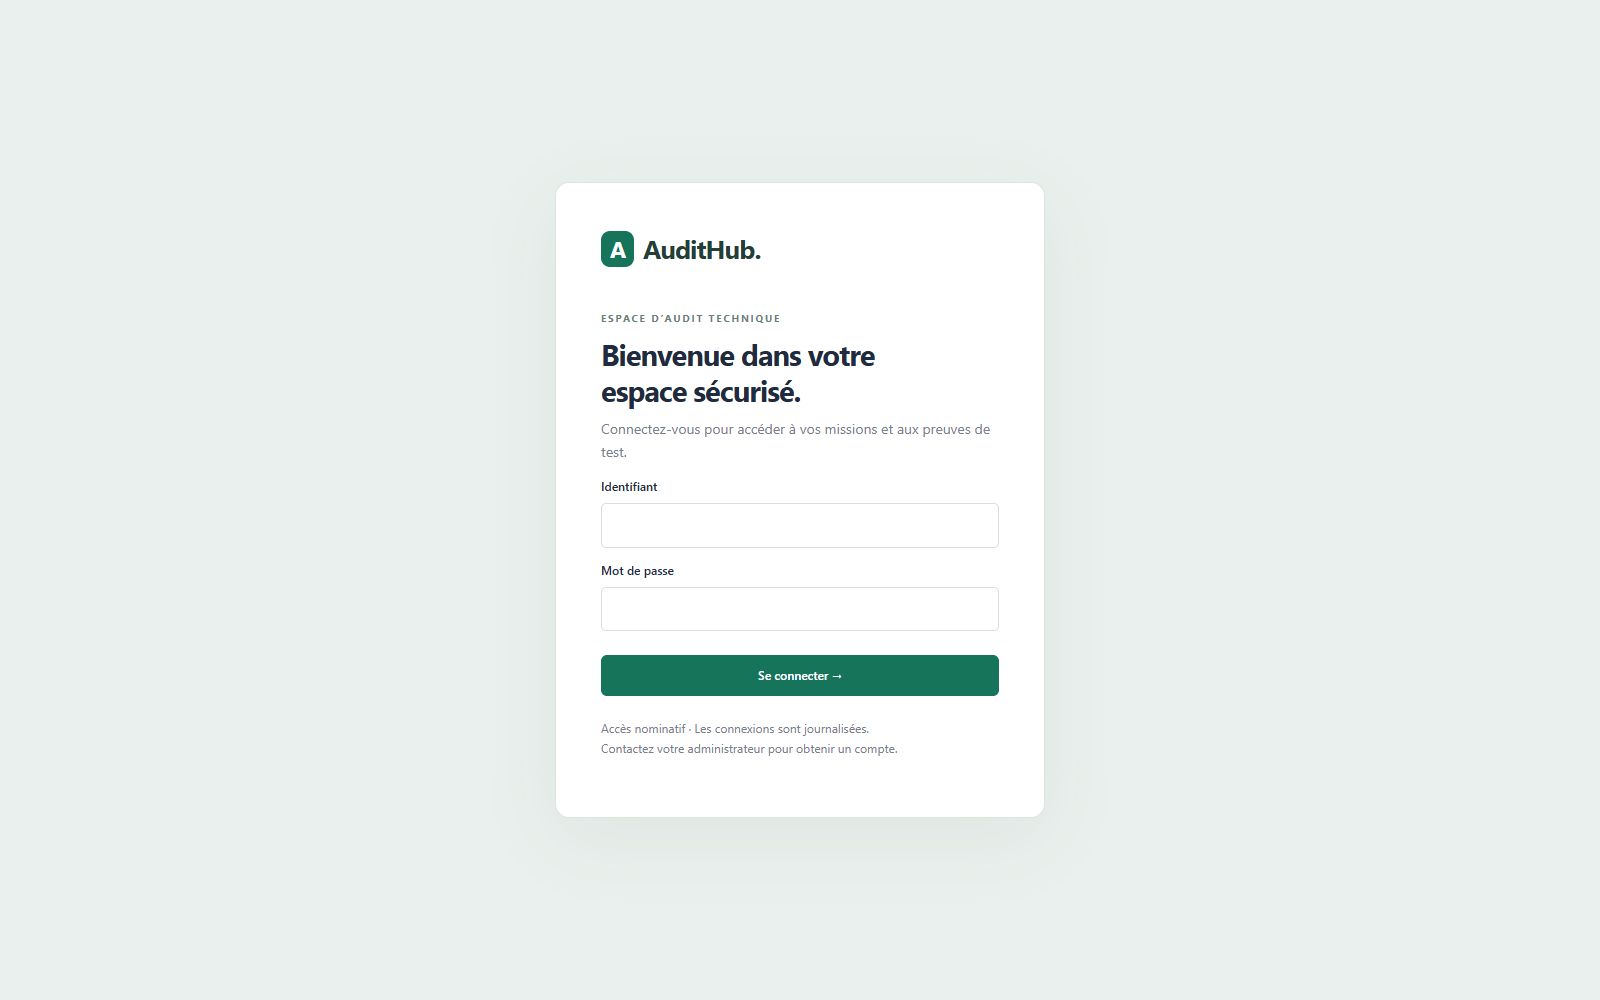
\includegraphics[width=.82\textwidth]{figures/screenshots/01-connexion.png}
\caption{Page de connexion r\'eelle d'AuditHub}
\label{fig:login}
\end{figure}

\begin{figure}[H]
\centering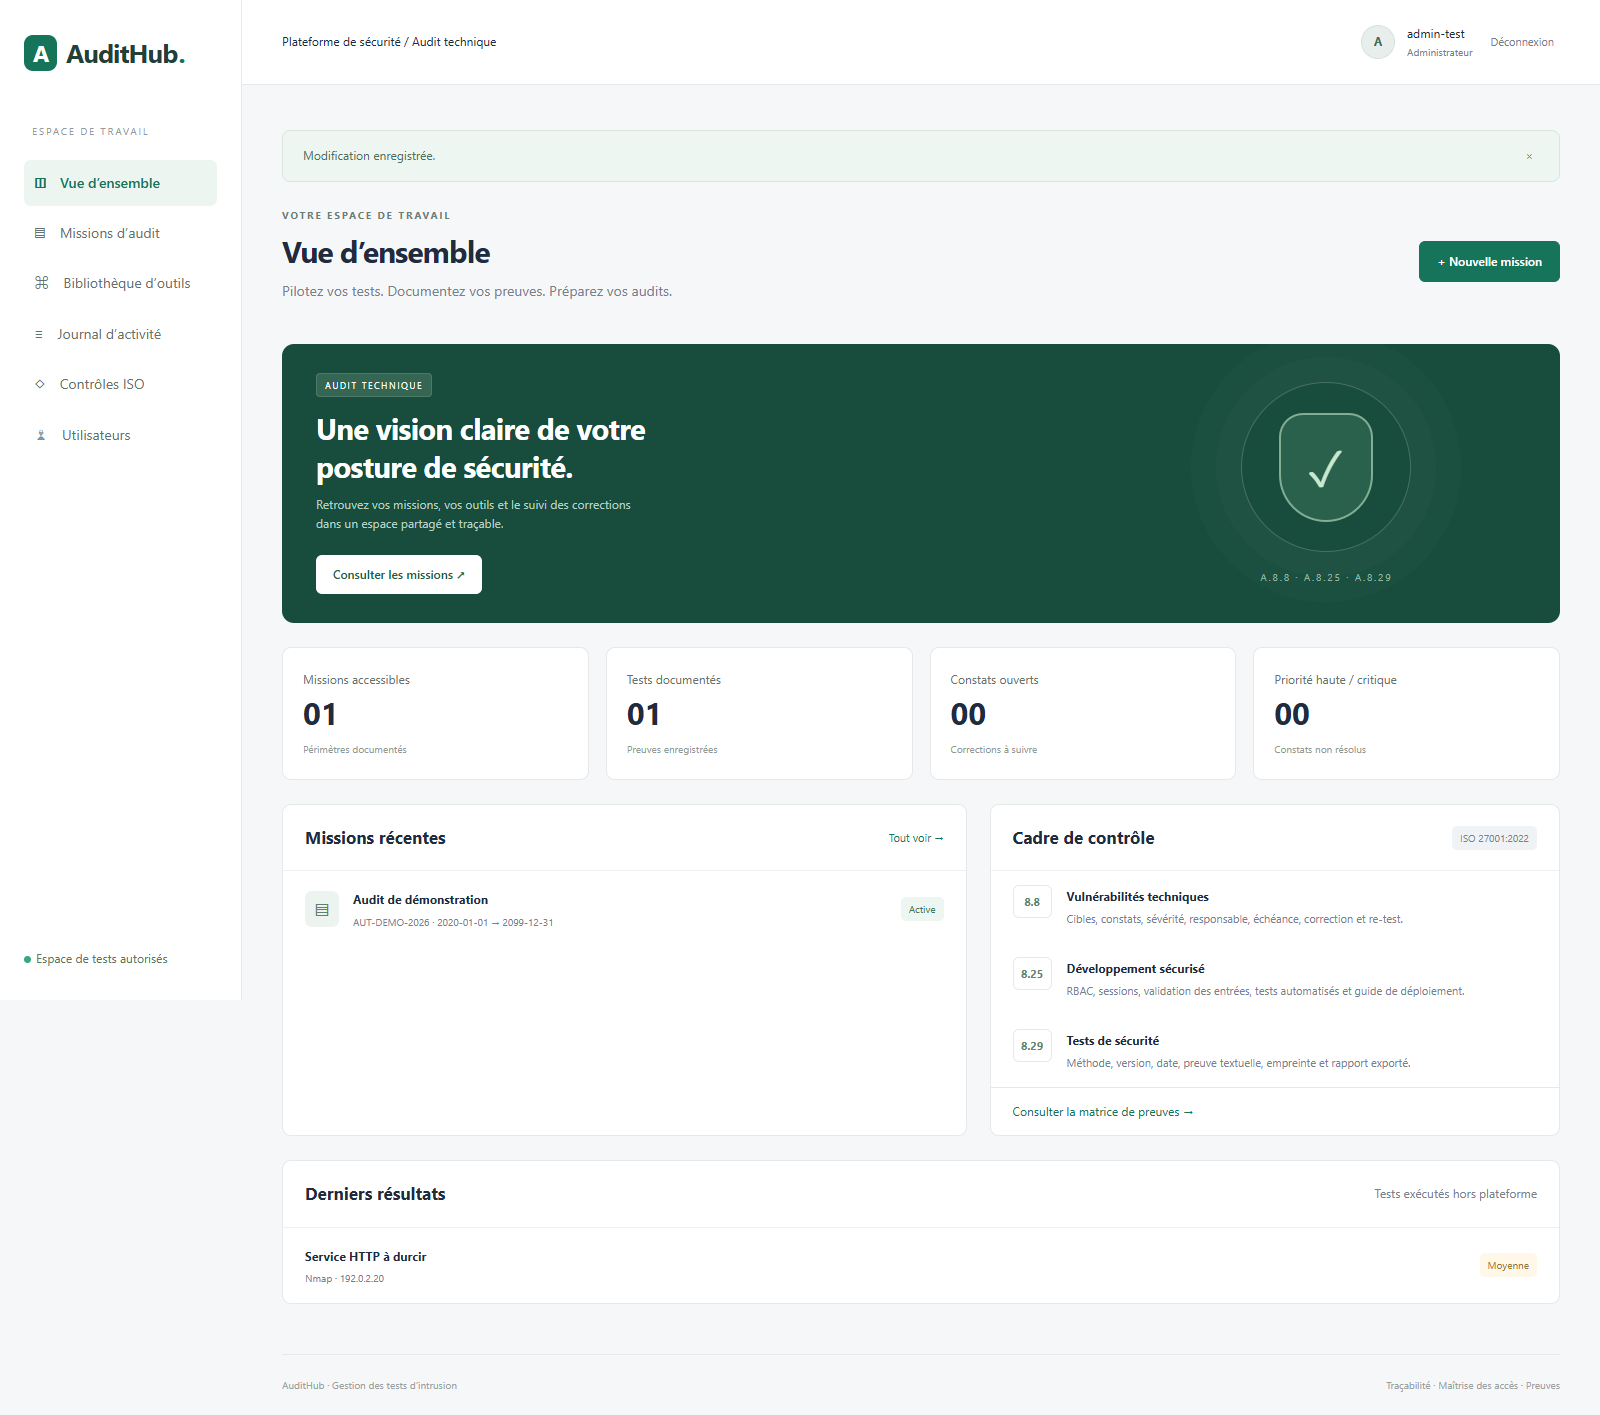
\includegraphics[width=.98\textwidth]{figures/screenshots/06-tableau-de-bord.png}
\caption{Tableau de bord aliment\'e par des donn\'ees synth\'etiques}
\label{fig:dashboard}
\end{figure}

\section*{D\'emonstration du flux d'audit}
\addcontentsline{toc}{section}{D\'emonstration du flux d'audit}
La campagne de capture cr\'ee une mission \og Audit de d\'emonstration \fg{} dans une base temporaire, lui associe un p\'erim\`etre IPv4/IPv6, consigne un constat Nmap, puis enregistre un re-test. Les informations sont synth\'etiques et n'exposent aucune donn\'ee de la base de travail.

\begin{figure}[H]
\centering
\begin{subfigure}{.48\textwidth}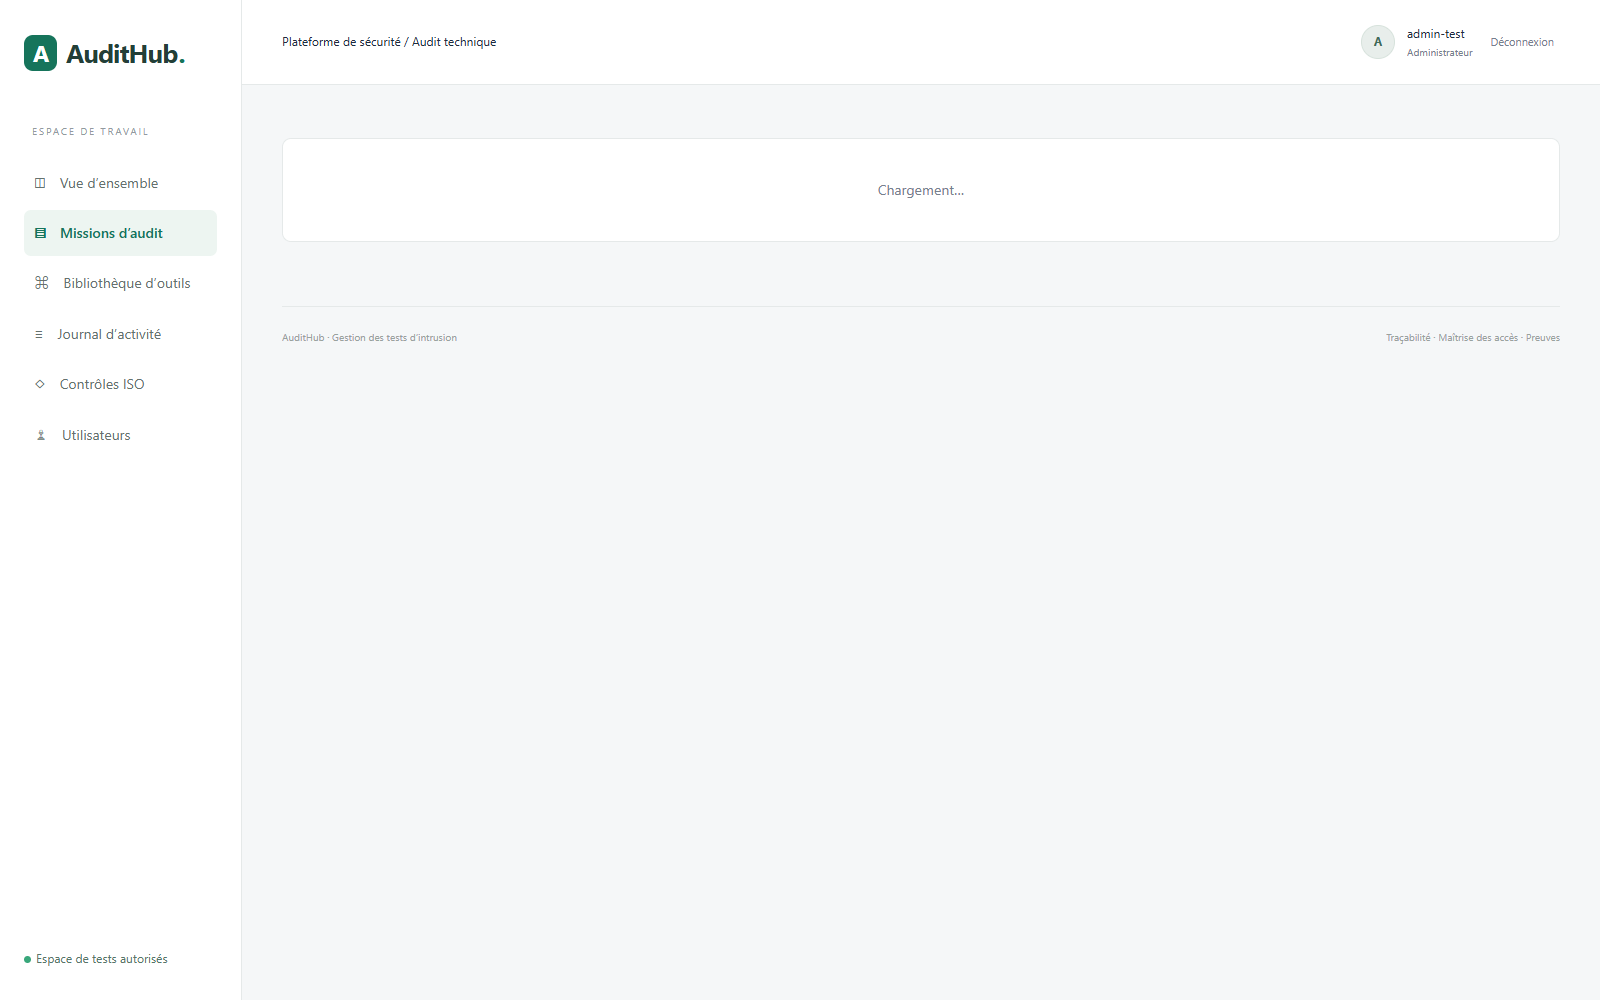
\includegraphics[width=\linewidth]{figures/screenshots/02-creation-mission.png}\caption{Formulaire de mission}\end{subfigure}\hfill
\begin{subfigure}{.48\textwidth}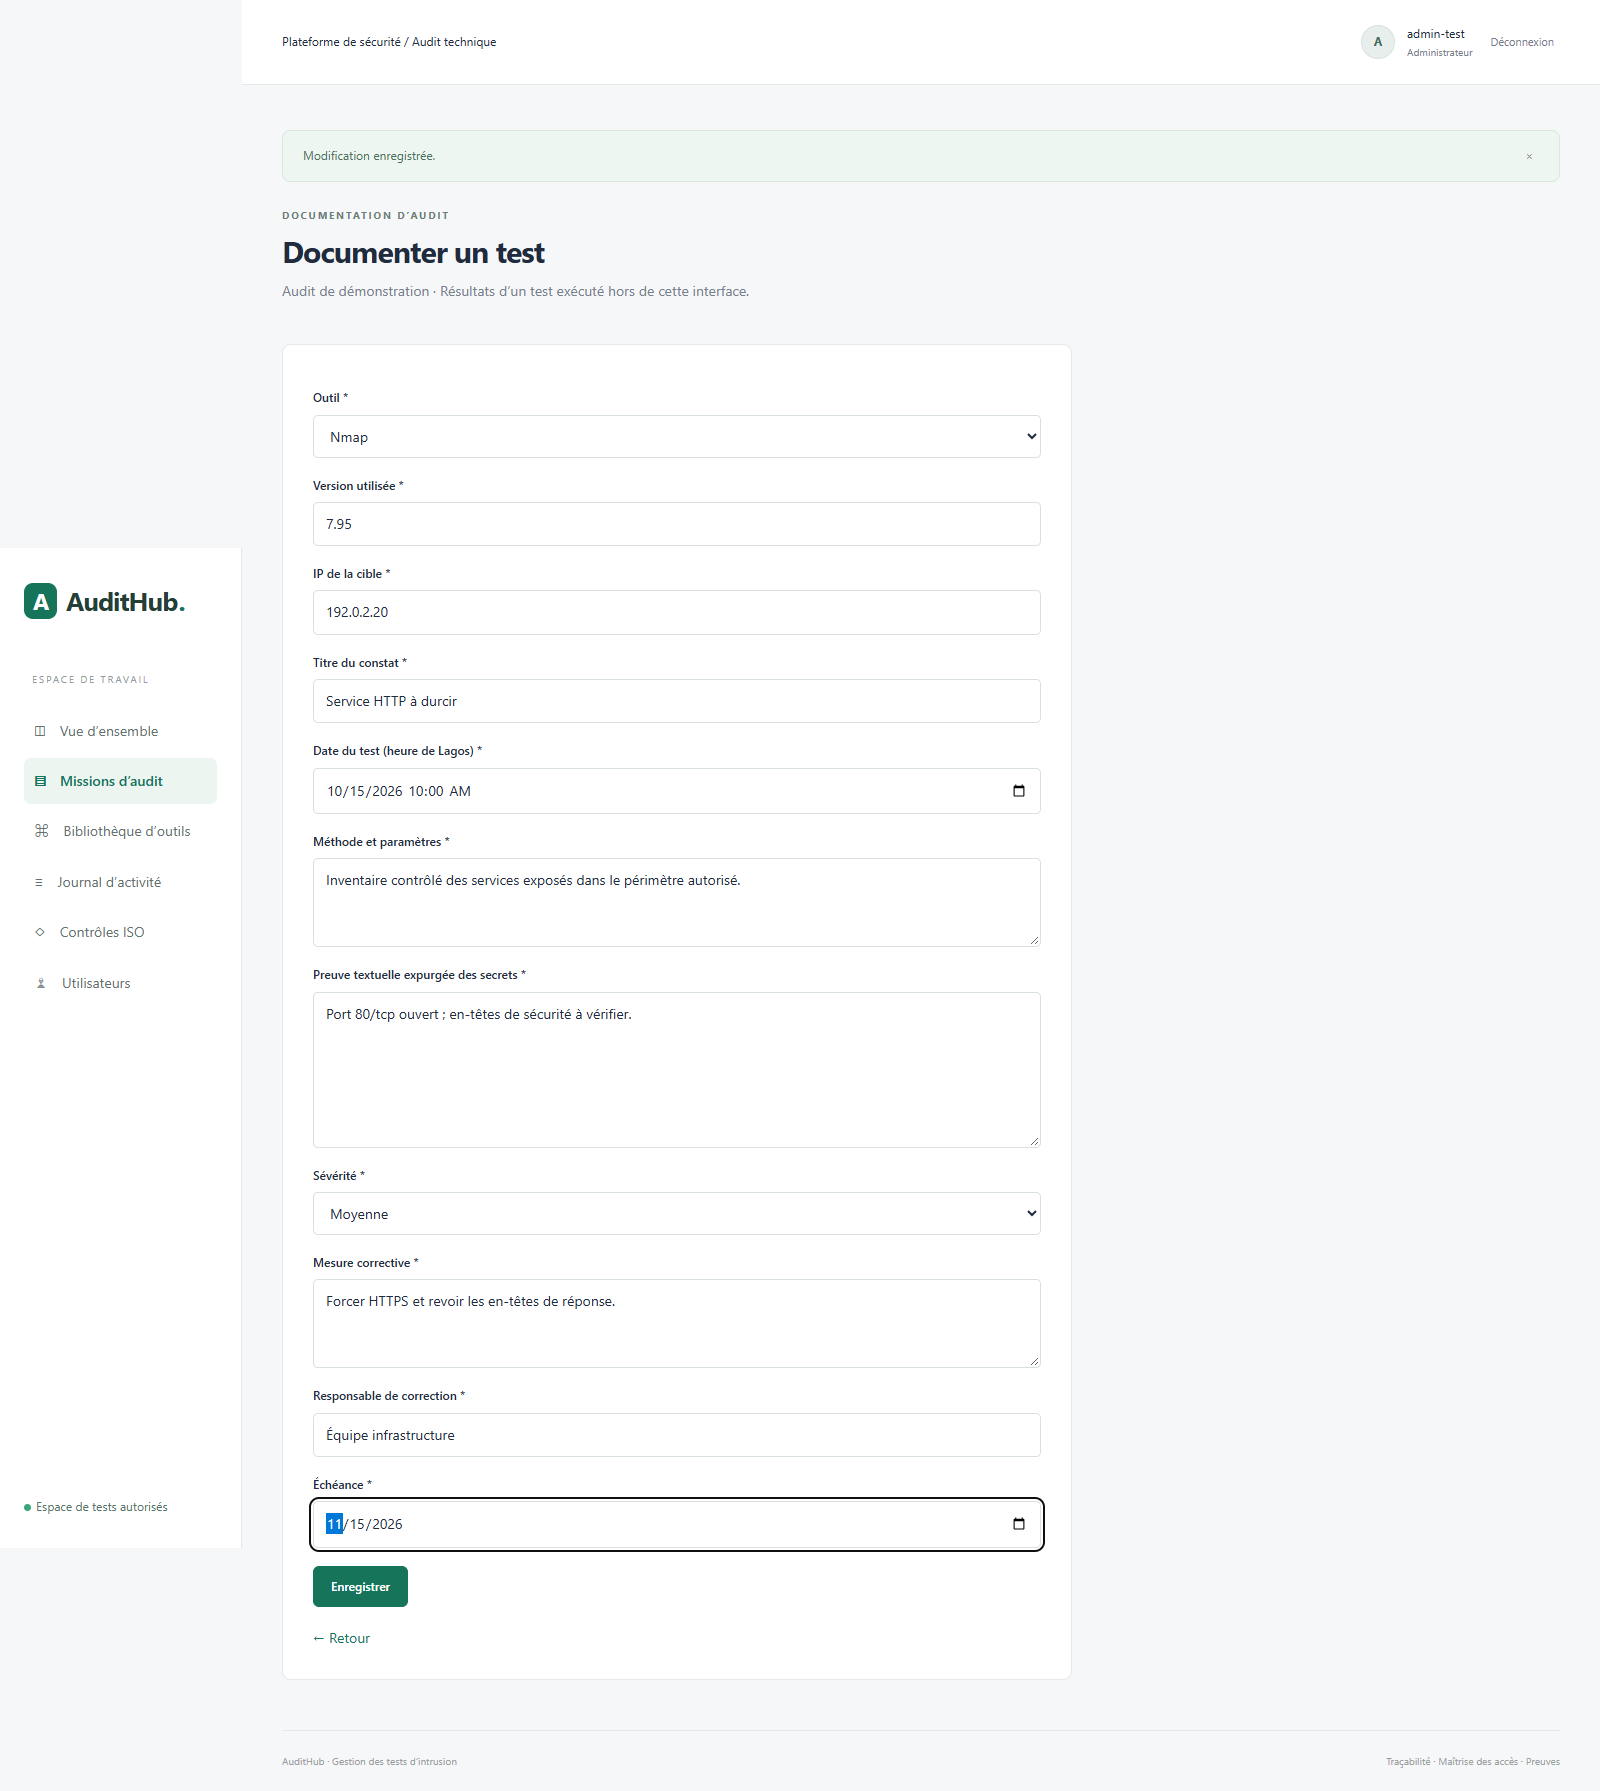
\includegraphics[width=\linewidth]{figures/screenshots/03-saisie-resultat.png}\caption{Saisie d'un r\'esultat}\end{subfigure}
\caption{Cr\'eation du p\'erim\`etre et documentation d'un test}
\label{fig:forms}
\end{figure}

\begin{figure}[H]
\centering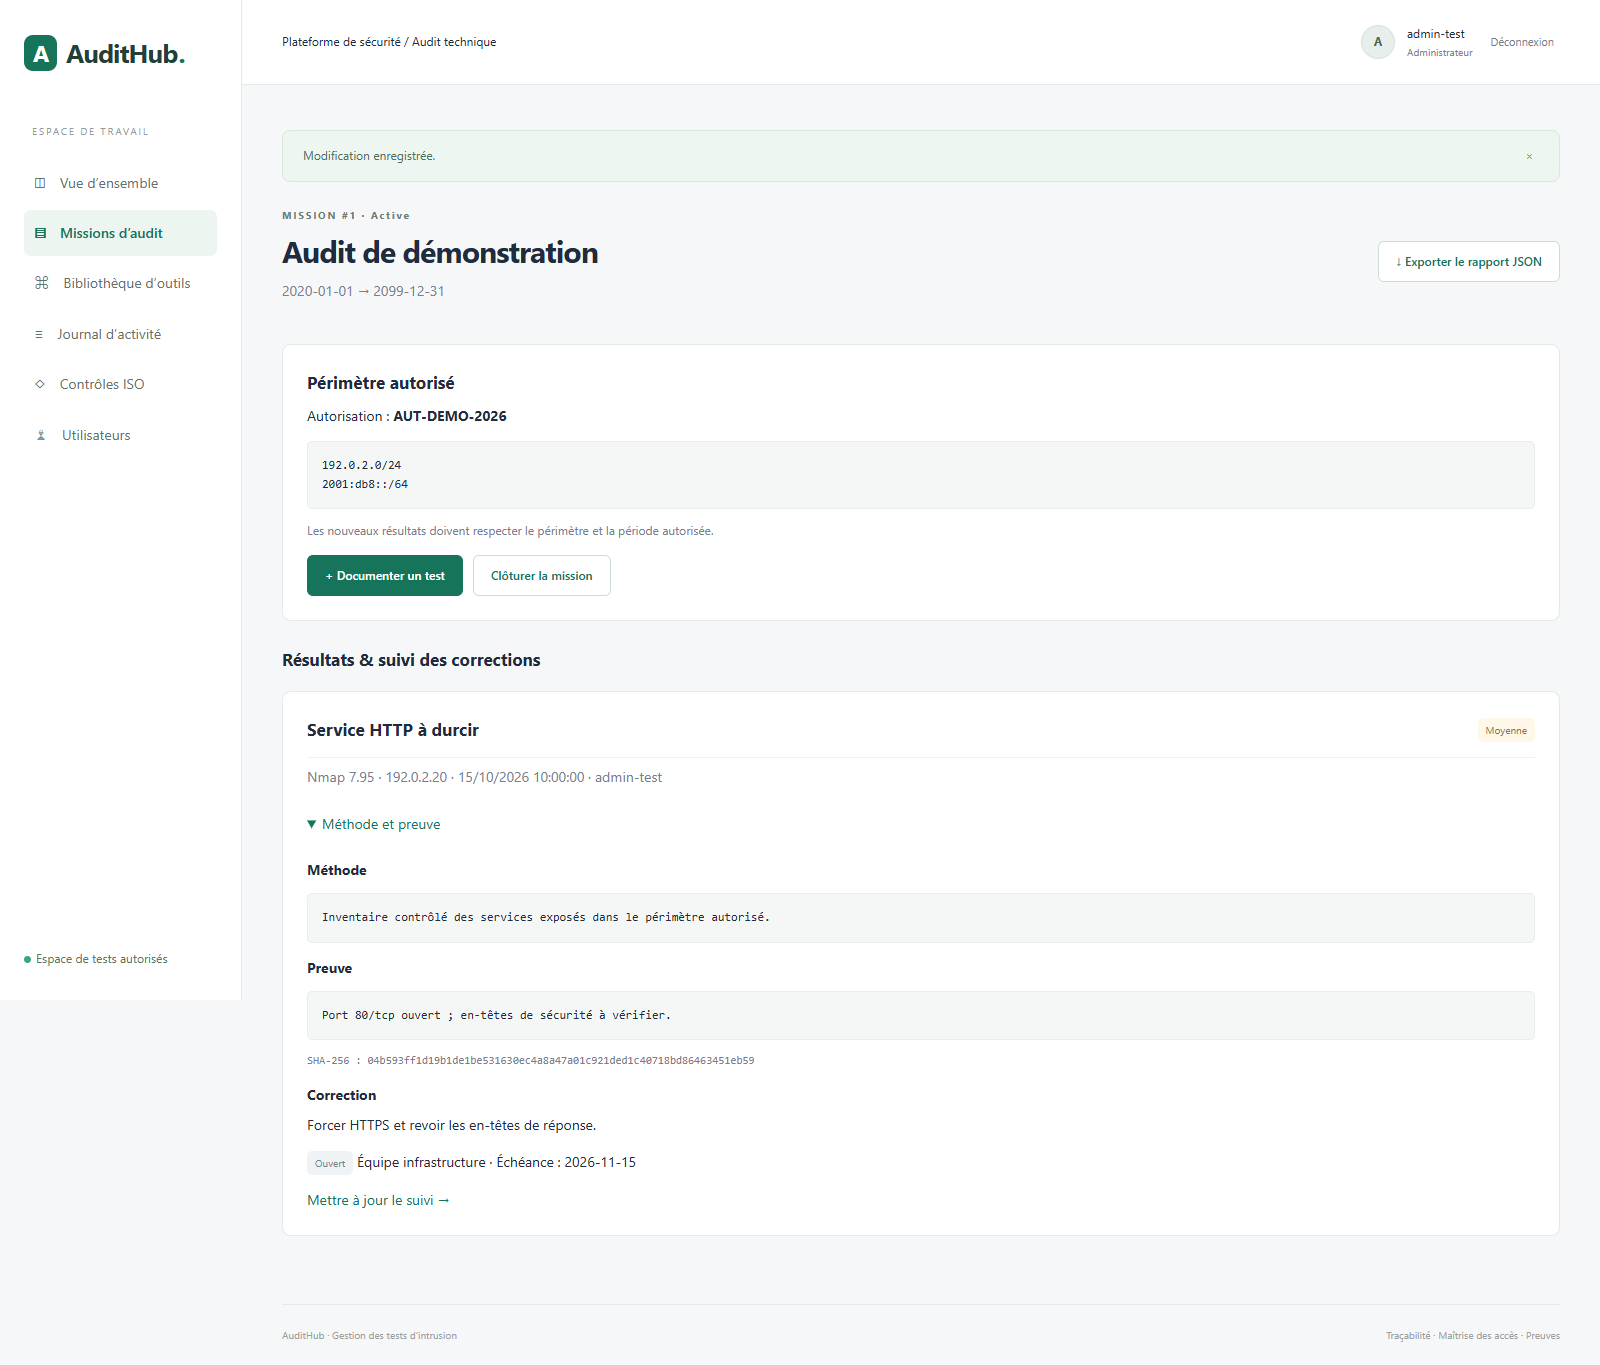
\includegraphics[width=.96\textwidth]{figures/screenshots/04-detail-mission.png}
\caption{D\'etail d'une mission avec preuve textuelle et empreinte SHA-256}
\label{fig:mission-detail}
\end{figure}

\begin{figure}[H]
\centering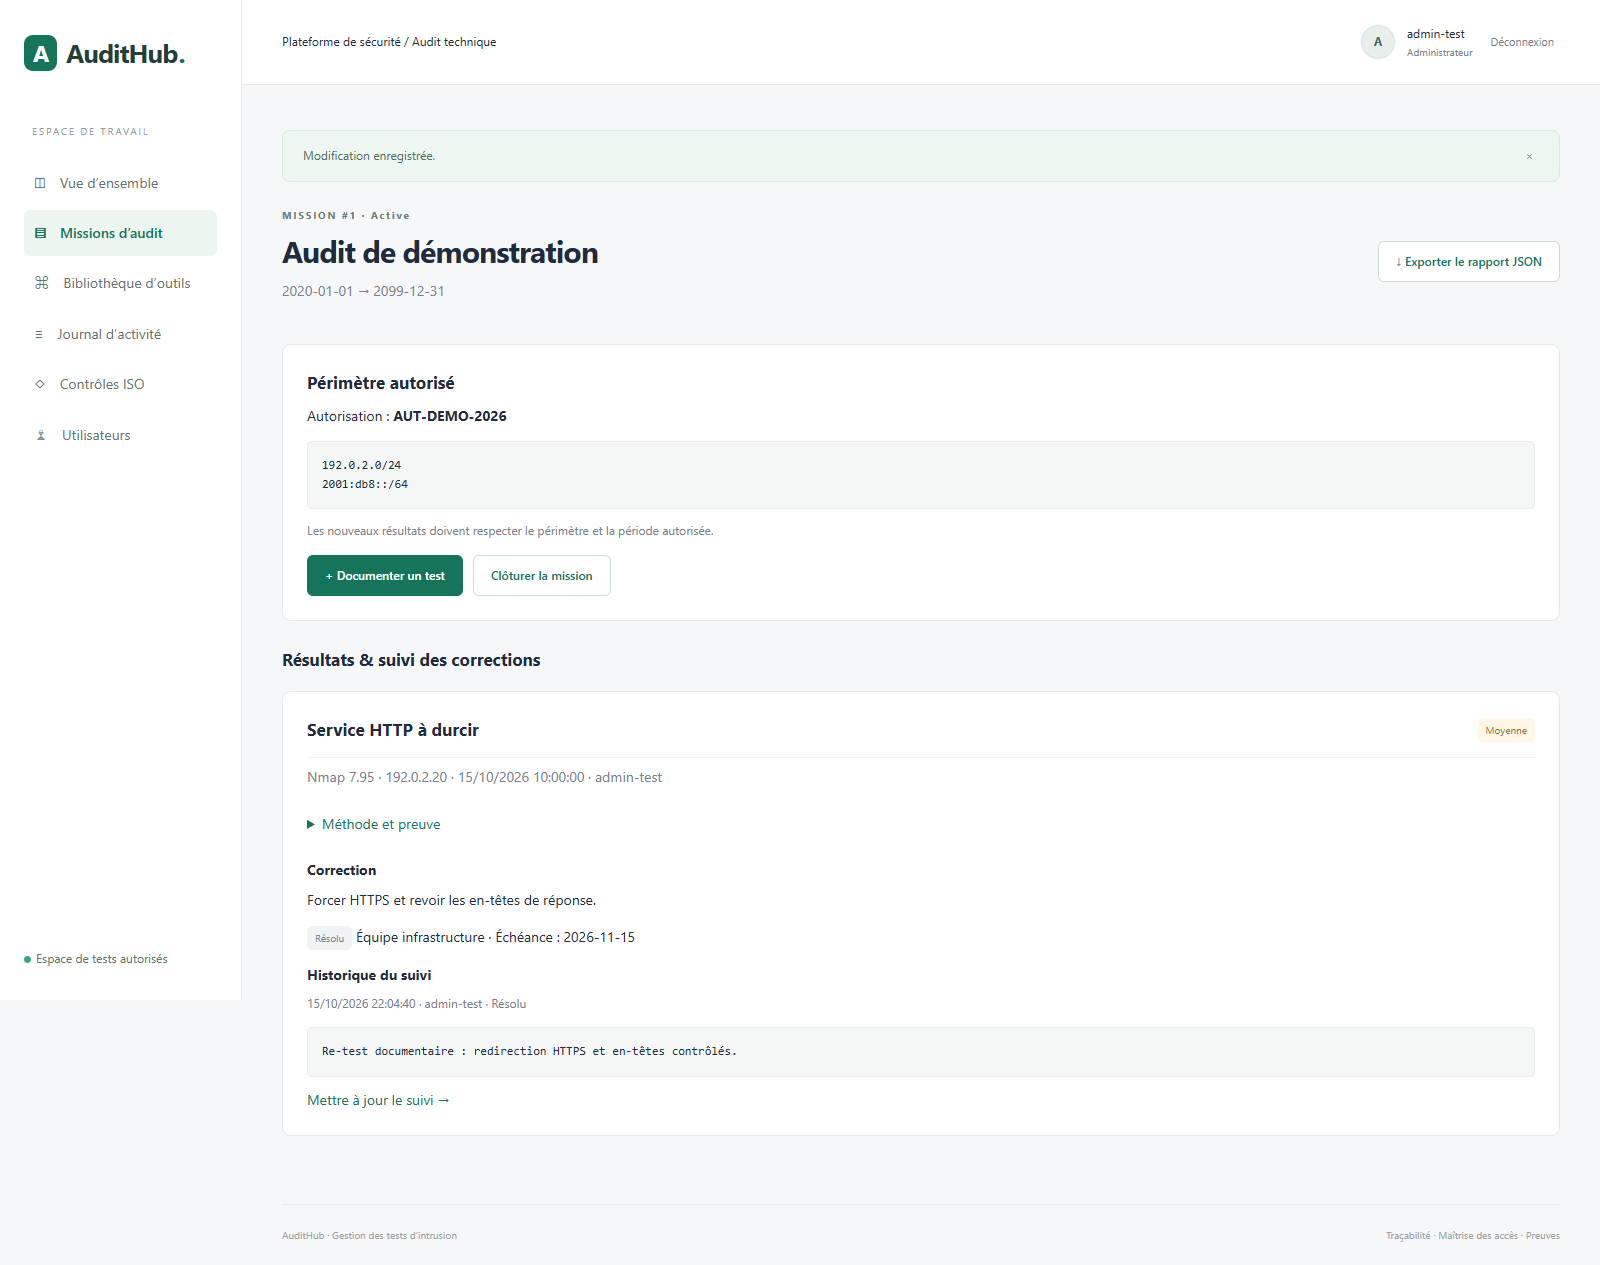
\includegraphics[width=.96\textwidth]{figures/screenshots/05-historique-suivi.png}
\caption{Historique dat\'e d'un suivi de correction}
\label{fig:followup}
\end{figure}

\section*{S\'ecurit\'e impl\'ement\'ee}
\addcontentsline{toc}{section}{S\'ecurit\'e impl\'ement\'ee}
\begin{itemize}
  \item mot de passe hach\'e par Django et validateurs imposant notamment 12 caract\`eres ;
  \item session de 30 minutes d'inactivit\'e, expiration \`a la fermeture, cookie HttpOnly et SameSite Strict ;
  \item cookies Secure, redirection HTTPS et HSTS hors mode d\'eveloppement ;
  \item jeton CSRF renouvel\'e apr\`es connexion et mutations POST ;
  \item CSP sans script inline/eval, refus du framing, politique de permissions restrictive et \evidence{no-store} ;
  \item limitation par compte (5 \`echecs) et par IP (30 \`echecs) sur 15 minutes ; les succ\`es ne consomment pas le quota ;
  \item filtrage des missions avant lecture, \`ecriture et export ;
  \item preuve initiale non modifiable dans l'interface et empreinte SHA-256 ;
  \item journalisation des actions sensibles et historique des suivis.
\end{itemize}
Ces mesures ne garantissent pas l'inviolabilit\'e face \`a un administrateur de base. L'empreinte stock\'ee avec la preuve n'est pas une signature externe.

\begin{figure}[H]
\centering
\begin{subfigure}{.48\textwidth}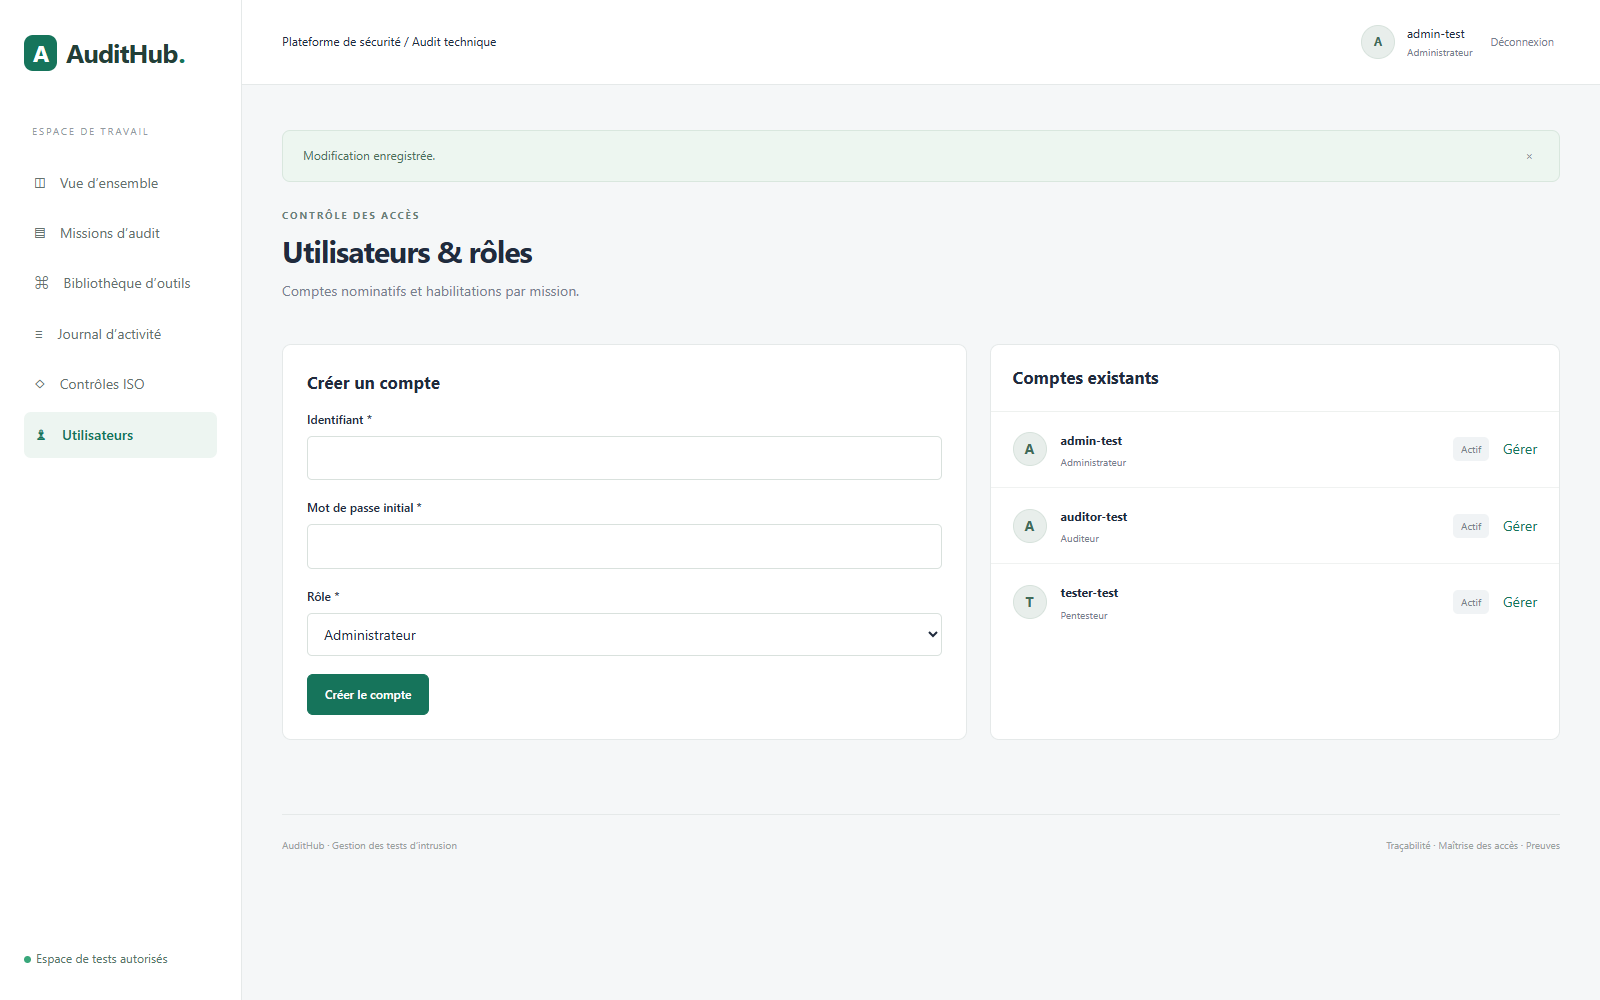
\includegraphics[width=\linewidth]{figures/screenshots/07-utilisateurs-roles.png}\caption{Comptes et r\^oles}\end{subfigure}\hfill
\begin{subfigure}{.48\textwidth}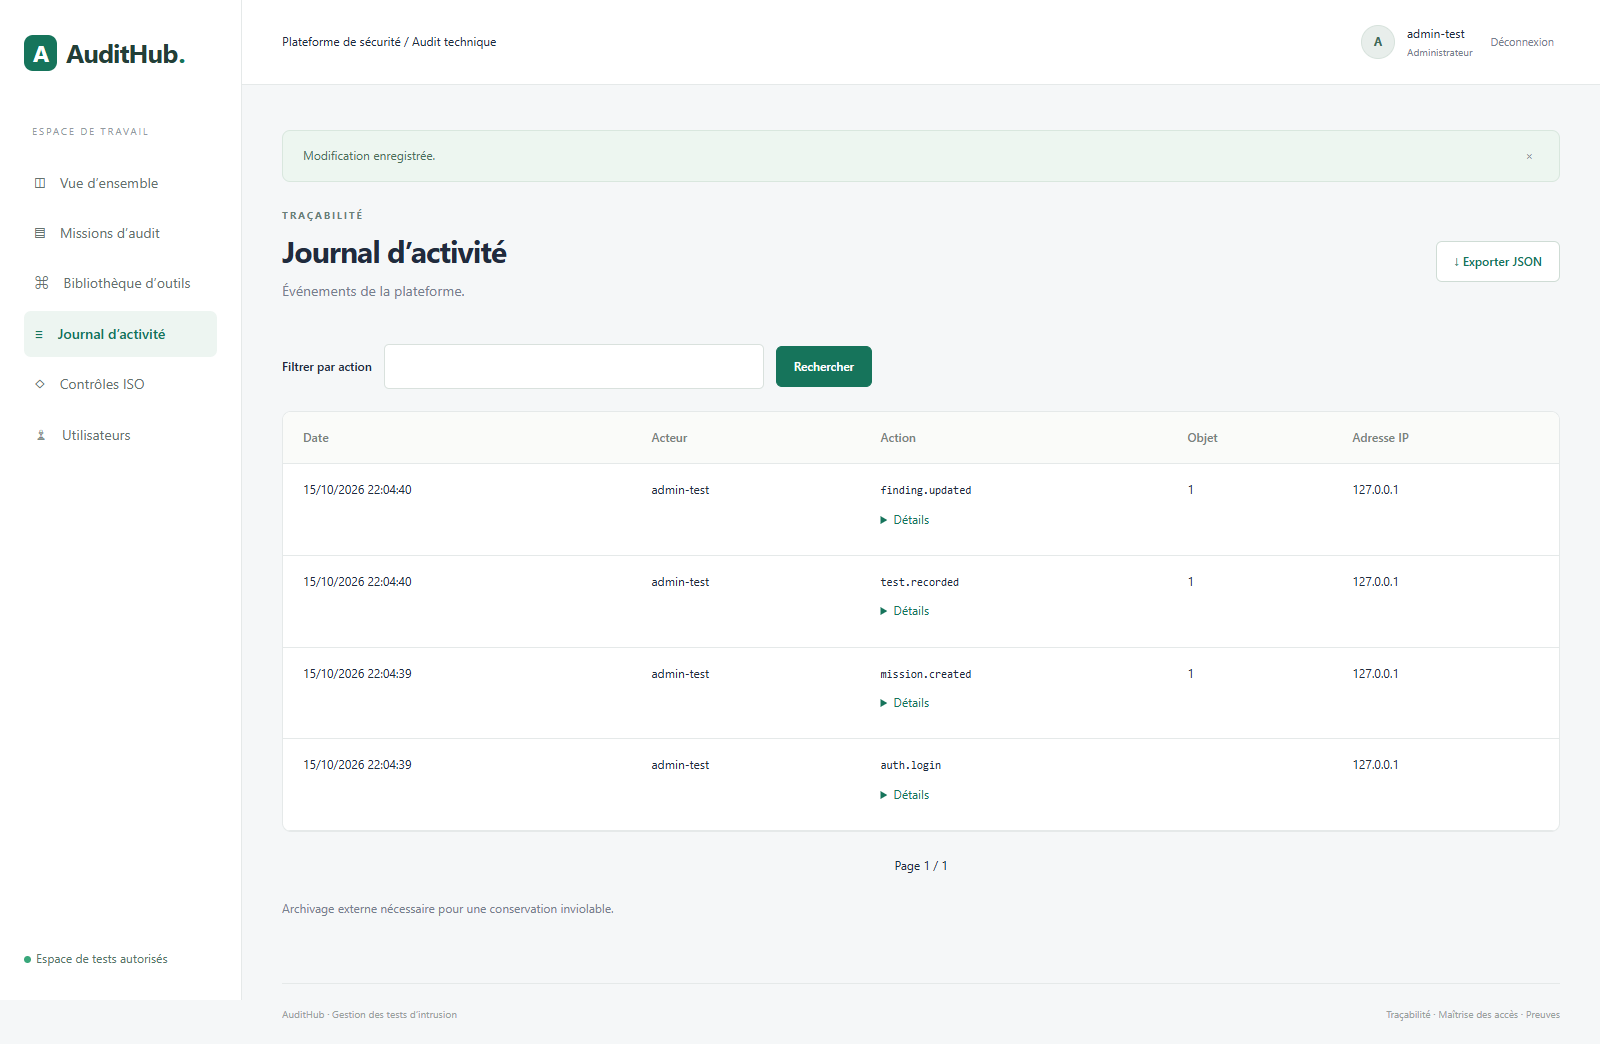
\includegraphics[width=\linewidth]{figures/screenshots/08-journal.png}\caption{Journal d'activit\'e}\end{subfigure}
\caption{Fonctions d'administration et de tra\c{c}abilit\'e}
\label{fig:admin-log}
\end{figure}
